\documentclass[a4paper]{article}

\usepackage{interspeech2013,amssymb,amsmath,epsfig}
\usepackage{booktabs}
\setcounter{page}{1}
\sloppy		% better line breaks
\ninept
%SM below a registered trademark definition
\def\reg{{\rm\ooalign{\hfil
     \raise.07ex\hbox{\scriptsize R}\hfil\crcr\mathhexbox20D}}}

%% \newcommand{\reg}{\textsuperscript{\textcircled{\textsc r}}}
\title{Understanding the Perception of Courteous and Humorous Behavior using Prosodic and Lexical Features}

\makeatletter
\def\name#1{\gdef\@name{#1\\}}
\makeatother
\name{{\em Sidd Jagadish$^\ast$, Ranjay Krishna$^\ddagger$, Gabriele Carotti-Sha$^\mp$}}
\address{{\small \tt siddj@stanford.edu, rak248@stanford.edu, gcarotti@stanford.edu}\\
$^\ast$Department of Statistics, Stanford University \\
  $^\ddagger$Department of Computer Science, Stanford University\\
  $^\mp$ Symbolic Systems, Stanford University\\
}

%
\begin{document}
\maketitle
%

\begin{abstract}
Computationally understanding the perception of a speaker's characteristics is an important task speech processing, behavioral outcomes and dialogue systems. Our work focuses on the classification and understanding the perception of two such characteristics: courtesy and humor. We analyze ratings surveyed from the SpeedDate corpus to build models using prosodic and lexical features of the speakers. We find that lexical features like \textit{Hedge-words} and prosodic features like \textit{Intensity Min SD} are important for detecting courteous while \textit{Exclamations} and listener's \textit{Intensity} are important for funny. Using an Adaboost Classifier, we detect the funny with an accuracy of SHIT GOES HERE and courteous at SHIT GOES HERE.\\

\end{abstract}

\noindent{\bf Index Terms}: Prosody, Speed Date, AdaBoost, Gender differences in prosody, factor analysis, courteous, funny

%

\section{Introduction}
Efforts in linguistic understanding encounter inevitable difficulties whether the interpretative entity is a human or a machine. For example, any communicative exchange across agents runs the risk of misrepresentation of one's self or of their interlocutor. It has been shown that given a dialogue between just two agents, human judgments about each other can be subject to great discrepancies (R. Ranganath et al. 2009), and this is potentially due to a failure in recognizing each other's affective cues. 
To face this issue, it is useful to invoke the notion of \textit{interpersonal stances}, as described by Schaerer (2000, 2003). An interpersonal stance is the way in which interlocutors pose themselves with respect to other agents within a given exchange. In particular, this notion incorporates affective stances, such as flirtatiousness, awkwardness, or courteousness, whose expression can be detected via subtle cues from a speaker's voice or words. This observation leads to the definition of two sets of communicative features: prosodic, pertaining to the physical characteristics of the vocal signal, and lexical, pertaining to the semantic content of the words pronounced. 

Examples of prosodic features are the fundamental frequency contour, or pitch, of a given speaker's voice, or the mean intensity they use to convey a particular emotive state (anger, excitement, humor). On the other hand, the number of times a given word is repeated, either throughout an entire conversation or only in response to a preceding speech segment, are considered lexical features. 
Thanks to the detailed and insightful research conducted by R. Ranganath et al. (2013), it has been possible to extract both sets of features from a series of speed date encounters, which were recorded and transcribed. Despite the relative artificiality of conversations within this particular context, this very artificiality can be favorable in an empirical study: it poses constraints on how much time interlocutors have to establish an exchange, and also generates very specific interpersonal stances (listed in the following sections), all of which are relevant to the date being either a success of a failure. By applying NLP classification methods to the extracted feature sets, it is possible to generate a fairly accurate predictor of whether, given a pair of interlocutors, one of the two found the other to be flirtatious, intelligent, etc. and vice versa. 

We build our own models upon the previously conducted research on the same dataset, and apply the same techniques in order to detect stances such as courteousness, sincerity, and humor.  

\section{Related Works}
Ranganath et al. (2013) use similar features, extracted from the same data, to predict the labels of awkwardness, friendliness, flirtatiousness, and assertiveness, finding that prosodic and linguistic features can indeed predict these labels quite well \cite{ranganath}.  In addition, they find that the mot relevant predictors vary significantly across labels and genders.  Ranganath et al. (2009) find that using stacked autoencoders to find low-dimension representations of the lexical data significantly improves prediction accuracies \cite{ranganath2}.   

\section{The SpeedDate Dataset}
We utilize the SpeedDate dataset introduced by \cite{jurafsky} to build our model. The dataset contains approximately 1100 heterosexual 4-minute speed dates. Each date is stored as a wav file recording of the speed date along with text files of the dates annotations. On average, each date contains 
812 words, with an average of 406 words per speaker. These worded are divided into an average of 93 turns per date where the speaker changes to the other.

\subsection{Feature Extraction}
We use OpenSMILE to extract Prosodic features from audio files of the speed date. Lexical features are extracted from the transcripts with the help of the LIWC dictionary.

\subsubsection{Prosodic Feature}
Prosodic features describe the speech of the speaker. In our model, we include features such as \textit{F0, intensity, RMS Amplitute, turn duration} and \textit{pitch}. For each of these different features, we calculate the \textit{min, max, standard deviation (SD), range, sd sd} and \textit{mean}.

\subsubsection{Lexical Feature}
Using LIWC, introduced by \cite{pennebaker}, we extract \textit{hedge words} like \textit{sort of} and \textit{I guess} that indicate uncertainty. We also gather \textit{meta} words that represent common words in the given speed date scenario and \textit{academic} words like \textit{PhD} and \textit{research}. Finally, we record occurrences of discourse markers.

\subsubsection{LIWC Feature}
We use the LIWC software to classify words into specific topic groups like \textit{love, hate, food, negate} and \textit{drink}. We count the word occurrences within each speed date for each of these word topics.

\subsubsection{Accomodation Feature}
\cite{natale}, \cite{ireland} and \cite{levitan} demonstrate through their work the convergence of vocal intensities between interlocutors. To capture this convergence, we extract features from a speaker that accommodate the previous speaker's speech. These features include the \textit{Rate of Speech} of the two speakers over time, the number of \textit{functional} and \textit{content} words also used in the other's previous turn and \textit{laughter} that immediately proceeds the other's laugh.

\subsection{Feature Normalization}
Before we use the features in our model, we normalize the relevant lexical feature with the the total word count in the conversation. We then normalize all the features such that they all have zero mean and unit variance.

\section{Exploratory Analysis}
Before attempting to classify speakers as funny or not, we examine the underlying dimensions along which the data varies.  To do, so we use exploratory factor analysis. To determine the number of factors, we use a scree test and various non-graphical measures, including parallel analysis and an optimal coordinates test, as described in (CITE).  We find an optimal number of factors $k = 5$ for both males and females, conducted separately.  Figure~\ref{scree} shows the two scree plots.

\begin{figure}[h]
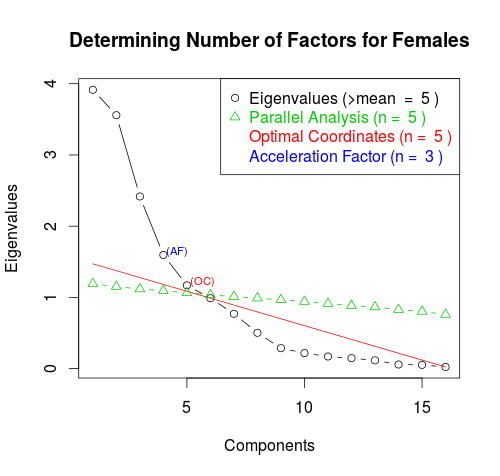
\includegraphics[width = 3.8cm]{graphics/ScreeFem.png}
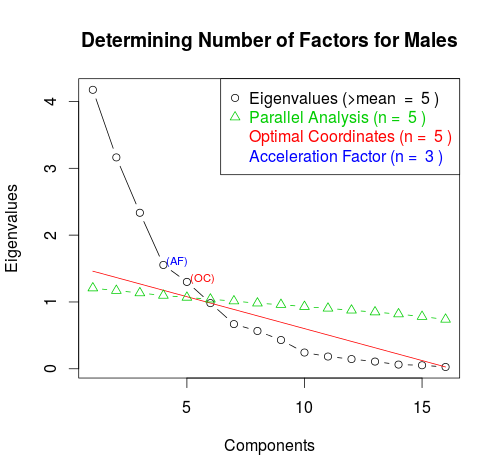
\includegraphics[width = 3.8cm]{graphics/ScreeMale.png}
\caption{{\it Determining Number of Factors}\label{scree}}  
\label{scree}
\end{figure}

\begin{table*} [t]
\centering
\begin{center}
\vspace{2mm}
\begin{tabular}{l | l l l l l l l l l l}
\hline
\multicolumn{1}{l}{\#} & 
\multicolumn{5}{c}{Male} &
\multicolumn{5}{c}{Female}\\
\cmidrule(r){2-6}
\cmidrule(r){7-11}
 Variable& Intens. & PitchMax& PitchMin & TurnDur & Intens.Var  &  PitchMax & Intens.Var  &  TurnDur  & PitchMin & Intens.Mean\\
 \hline
 tndur.mean & 0.03  & 0.26  & -0.22 & 0.94 & -0.05 & 0.17 & -0.03 & 0.97 & -0.15 & 0.04\\
 pmin.mean & 0.16 & -0.23 & 0.85 & -0.24 & 0.11 & -0.21 & -0.07 & -0.21 & 0.89 & 0.07 \\
 pmax.mean& 0.13& 0.94 & 0.01 & 0.23 & 0.0 & 0.92 & 0.03 & 0.23 & -0.1 & 0.05 \\
 pmean.mean& 0.18 & 0.53 & 0.69 & -0.13 & 0.07 & 0.72 & -0.02 & 0.02 & 0.48 & 0.19 \\
 psd.mean& -0.12 & 0.71 & -0.38& -0.06 & 0.01 & 0.88 & 0.09 & -0.11 & -0.28 & -0.05\\
 imin.mean& 0.54 & 0.09 & 0.13 & -0.27 & -0.21 & -0.02 & -0.75 & -0.06 & 0.07 & 0.46\\
 imax.mean& 0.93& 0.13 & 0.06& 0.19 & 0.0 & 0.1 & -0.16 & 0.06 & 0.03 & 0.9\\
 imean.mean& 0.99& 0.05& 0.12& 0.06 & -0.02 & 0.07 & -0.48 & -0.01 & 0.1 & 0.87\\
 tndur.sd& 0.00& 0.12& -0.1 & 0.87 & -0.04 & 0.05 & 0.04 & 0.87 & -0.04 & 0.03\\
 pmin.sd & 0.01& -0.03 & 0.83 & -0.07 & 0.16 & -0.06 & 0.02 & -0.09 & 0.87 & 0.02\\
 pmax.sd& -0.12 & -0.78 & -0.09 & -0.17 & 0.08  & -0.67 & 0.01 & -0.1 & 0 & -0.05\\
 pmean.sd& -0.09& -0.04 & 0.13 & -0.16 & 0.27 & 0.11 & 0.11 & -0.3 & 0.3 & 0.03\\
 psd.sd& -0.20& -0.42 & -0.01 & -0.28 & 0.21 & -0.27 & 0.06 & -0.33 & 0.12 & -0.01\\
 imin.sd& 0.07 & 0.00 & 0.02 & 0.02 & 0.36 & 0.0 & 0.36 & 0.03 & 0.14 & 0.02\\
 imax.sd& -0.65 & -0.08 & 0.07 & -0.06 & 0.66 & 0.0 & 0.87 & -0.12 & -0.07 & -0.35\\
 imean.sd& -0.27 & -0.09 & 0.12 & -0.01 & 0.95 & 0.04 & 0.97 & -0.14 & -0.11 & -0.12\\
 Var Explained& 0.18 & 0.16 & 0.13 & 0.13 & 0.10 & 0.17 & 0.17 & 0.13 & 0.13 & 0.12\\
 \hline
\end{tabular}
\caption{\label{table:Factor Analysis} {\it  Factor Analysis Loadings Matrices}}
\end{center}
\label{table:results}
\end{table*}

Interestingly, although we find that the various factors for male and female speech are similar, they explain different amounts of variation in the data.  For males, the first factor reflects high intensity values and low intensity variation, explaining   

\section{Evaluation Approach}

\subsection{Methodology}
We divide the dataset into two separate groups based on gender. For each gender, we train a classifier for detecting the perception of funny and courteous characteristics.  

We create a training set for a given characteristic for a given gender by splitting the dataset into deciles. We use the top decile as positive and the bottom decile as negative examples. 

\subsection{Classifiers}
We start by using an SVM with a linear kernel. To improve our classifications, we next enforce an L1 norm on the SVM to compensate for the large number of lexical and prosodic features we extract. In case our decision boundaries are non-linear, we also train a RBF kernelized SVM. However, we lose interpretability of the features by using an RBF. So, we train a fourth Adaboost Classifier with decision stumps of unary depth to maintain interpretability while also allowing for a non-linear decision boundary. 

\section{Classification Results}
\begin{table*} [t]
\centering
\begin{center}
\vspace{2mm}
\begin{tabular}{l l l| l l l l l l l l}
\hline
\multicolumn{1}{l}{Participant} & 
\multicolumn{1}{l}{Gender} &
\multicolumn{1}{l}{Predictors} &
\multicolumn{4}{c}{Funny} &
\multicolumn{4}{c}{Courteous}\\
\cmidrule(r){1-3}
\cmidrule(r){4-7}
\cmidrule(r){8-11}
&  & & SVM RBF & SVM Lin & AdaBoost & L1SVM & SVM RBF & SVM Lin & AdaBoost & L1SVM\\
\hline
 Male & Both & Prosody & 0.70 & 0.69 & 0.66 & 0.65 & 0.71 & 0.68 & 0.70 & 0.66\\
 Male & Self & Lexical & 0.64 & 0.59 & 0.59 & 0.61 & 0.63 & 0.61 & 0.64 & 0.63\\ Male & Both & Lexical & 0.63 & 0.57 & 0.61 & 0.55 & 0.65 & 0.61 & 0.65 & 0.65\\
\\
 \\
  \\
  \\
  \\
 \\
 \\
 \\
 \hline
\end{tabular}
\caption{\label{table:results} {\it  Classification Results.}}
\end{center}
\label{table:results}
\end{table*}

First, we run our four classifiers on our prosodic features only.  Despite only looking at acoustic features of these conversations, we achieve promising results -- an accuracy of 71.2\% for courteousness and 69.8\% for funniness.  These results are shown in Table~\ref{table:results}

\section{Analysis}

\subsection{Adaboost Weights}
By limiting the depth of the trees in Adaboost to 1, we are able to unravel the top features that were used by each tree in Adaboost. We aggregate these top features by summing across the weights associated with each tree split to capture the features with the highest weights.

Since Adaboost learns different classifier each time, we perform a 10 fold feature aggregation and averaging the sum of weights for each feature split. We perform this aggregation by training on lexical and prosodic features independently. Table~\ref{table:adaboost} shows the top features that adaboost splits on. In the table, \textit{Other} refers to the listener's features.

\begin{table*} [t]
\centering
\begin{center}
\vspace{2mm}
\begin{tabular}{c l l l l}
\hline
\multicolumn{1}{l}{\#} & 
\multicolumn{2}{c}{Funny} &
\multicolumn{2}{c}{Courteous}\\
\cmidrule(r){2-3}
\cmidrule(r){4-5}
 & Lexical & Prosodic  & Lexical & Prosodic\\
 \hline
 1 & Other hear & Other imin SD & syllables per turn & imax mean \\
 2 & Other youKnow & Other pslope mean & probably & Other prange mean \\
 3 & Other see & tndur SD & like & Other pmin SD \\
 4 & Other achieve & Other tndur SD & relativ & ptmax SD \\
 5 & Other LaughAcc & Other pslnjmp mean & Other you know & itmin SD \\
 6 & syllables per turn & tndur mean & humans & Other pslnjmp mean \\
 7 & program & pquan mean & cogmech & Other.imin.SD \\
 8 & Other past & imax mean & sad & pquan mean \\
 9 & program & Other tndur mean & Other anxious & ptmin SD \\
 10 & Other pronoun & Other pmax mean & i think & iquan mean \\
 \hline
\end{tabular}
\caption{\label{table:adaboost} {\it  Feature Splits with Highest Weights in Adaboost.}}
\end{center}
\label{table:results}
\end{table*}

\subsubsection{Funny}
Based on the results for funny, words related the other person using words in the LIWC categories \textit{hear, youKnow, see} and \textit{achieve} are good indicators that the other person finds the speaker funny. The \textit{achieve} category correspond to words like \'win\' that has been expressed by the listener after the speaker delivers a joke. Words corresponding to \textit{hear} and \textit{see} demonstrate that the listener it paying attention and acknowledging the speaker's speech. The 5$^{th}$ feature is laughter accommodation where the listener laughs in reaction to the speaker's laugh.  

The prosodic features for funny also correspond well with the lexical features as shorter \textit{turn duration}, which is the 4$^{th}$ and 5$^{th}$ on the prosodic features list, between the two people usually results in more words in the LIWC \textit{see} and \textit{hear} categories of acknowledgement. These features also show that a high intensity min SD from the listener and a high pitch slope mean are good indicators of funny.

\subsubsection{Courteous}
Discourse words like \textit{like, probably and I think} are good lexical indicators for detecting courteous. The honesty weakening of there sentences by using such words makes them appear more courteous. Also, talking about \textit{humans} and \textit{cognitive processes} are important. The use of \text{anxious} and \textit{fillers} like \textit{you know} are the only features of the listener that have a high weight.

Low intensity max mean with small pitch range SD and pitch min SD are important prosodic features. This implies that large changes in speech are perceived as non being courteous.

\subsubsection{Comparing Funny and Courteous}
It is interesting to note that the speaker's features are the most important when determining whether the speaker will be perceived as courteous. On the other hand, the listeners features are more important for detecting funny.

\section{Future Work}
The model we build has a lot of features and reducing dimensionality of this data by learning hidden variables from an sparse auto-encoder might give us more insight into how we can create a shared representation of the lexical with the prosodic features.

The SpeedDate dataset we use also contains ratings of people's intelligence, sincerity and other characteristics. An interesting area to explore would find correlations between these characteristics and their corresponding prosodic and lexical features.

Adding another source of features, such as video from video speed dates is another extension to this project. It would be insightful to see how the contribution of the current features will change if visual features are also added.

\section{Conclusions}


\section{Acknowledgements}
We thank Dan Jurafsky for giving us access to the Speed Dating Dataset and for his continued guidance during this project.

\newpage
%
\eightpt
\bibliographystyle{IEEEtran}
\begin{thebibliography}{10}

\bibitem{jurafsky}Ranganatha, R., Jurafsky, D., McFarland, D.A., ``Detecting friendly, flirtatious, awkward, and assertive speech in speed-dates``, in Computer Speech \& Language
Volume 27, Issue 1, Pages 89-115, 2013

\bibitem{pennebaker}Pennebaker, J. W., Booth, R., Francis, M., ``Linguistic inquiry and word count: LIWC2007`` � operator�s manual. Tech. rep., University of Texas, 2007

\bibitem{natale}Natale, M.,  ``Convergence of mean vocal intensity in dyadic communication as a function of social desirability``, in Journal of Personality and
Social Psychology 32 (5), 790-804, 1975

\bibitem{ireland}Ireland, M.E., Slatcher, R.B., Eastwick, P.W., Scissors, L.E., Finkel, E.J., Pennebaker, J.W., ``Language style matching predicts relationship
initiation and stability``, in Psychological Science 22 (1), 39, 2011

\bibitem{levitan}Levitan, R., Hirschberg, J., ``Measuring acoustic-prosodic entrainment with respect to multiple levels and dimensions``, in ACL 2011

\bibitem{ranganath}Ranganath, R., Jurafsky, D., McFarland, D. ``It's Not You, It's Me'', in Proceedings of the 2009 Conference on Empirical Methods in Natural Language Processing.

\end{thebibliography}
\end{document}
